\chapter{応用例}
\label{chap:usage}

本章では、HypAR Touchによって実現可能な応用例について述べる。

\newpage


\section{駅など公共施設での案内}
駅や空港などの比較的大規模な公共施設内ではGPSによる案内が利用できないことが多く、地図を提示するか矢印などによる案内表示が一般的である。
地図は設置できる場所に限りがあるだけでなく、位置関係が複雑な場合は地図を見ただけでその構造を理解することは難しく、目的地にたどり着くのが難しいという問題点を持つ。
また案内表示の場合、記述できる情報に限りがあり、必ずしも自分の目的地に沿う案内があるとは限らないという問題点がある。

一方本システムではARで目的地を直接提示(図:\ref{fig:ar_navigation_shonandai})するため地図の苦手な人への案内や複雑な構造の施設の案内において有用である。
また壁など設置された小さなNFCタグに触れるだけでその場所からの案内を開始できるため設置場所にこまることがない。
さらにNFCタグは一枚あたり十数円と安価であるため設置数とコストに困ることは少ないと言える。
またNFCタグに紐付いた情報により表示するAR情報のあるScrapboxプロジェクトとやハイパーリンクによるフィルターを指定できるので用途に特化した案内(図:\ref{fig:ar_navigation_exit})をすることも可能である。

\begin{figure}[h]
  \begin{minipage}{0.5\hsize}
    \centering
    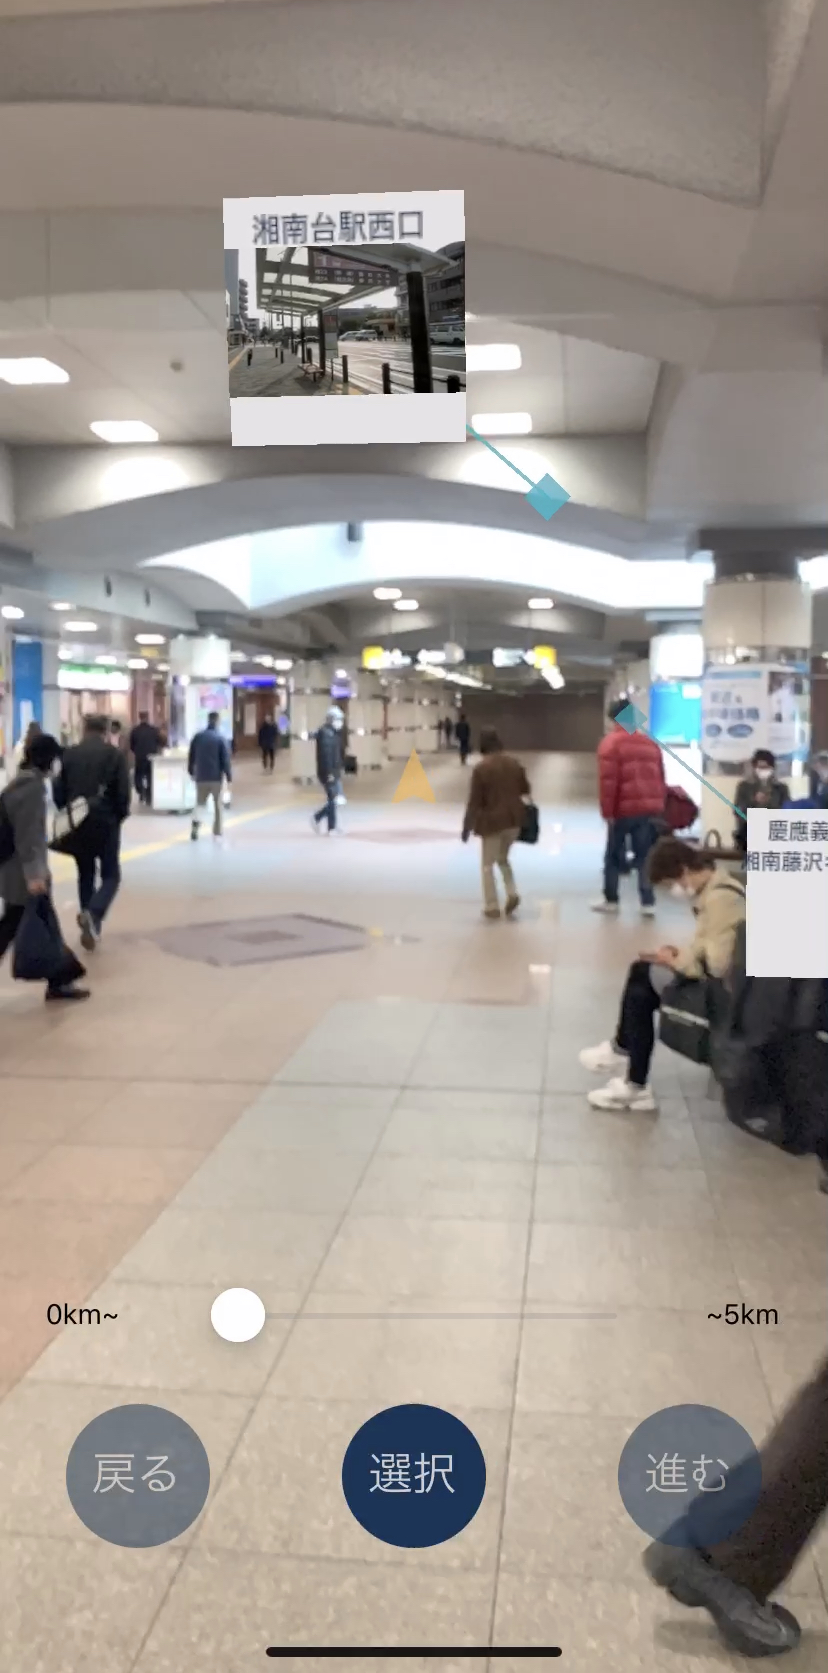
\includegraphics[width=70mm]{images/ar_navigation_shonandai.jpg}
    \caption{案内の様子} \label{fig:ar_navigation_shonandai}
  \end{minipage}
  \begin{minipage}{0.5\hsize}
    \centering
    
\includegraphics[width=70mm]{images/wip2.jpg}
    \caption{出口だけの案内} \label{fig:ar_navigation_exit}
  \end{minipage}
\end{figure}

\section{近隣施設の探索・推薦}
本システムの大きな特徴としてwikiを利用することにより情報を階層化せずに関連情報を探索できる点が挙げられる。
自分の興味のある近隣施設をリンクによって探索することが可能になっている。

例えば神保町で本システムを利用した場合、ウィンタースポーツ用品店を選択すれば、「スノーボード」「スキー」といったいったリンクが出現する(図\ref{fig:ar_navigation_jibotyo_ski})。
ウィンタースポーツ用品店を周りたい場合はこれらのリンクを選択することでウィンタースポーツに関連する施設の情報を見ることができる。

またその後食事をを取りたくなった場合は同じタグにタッチし飲食店をクリックすることで「ラーメン」「カレー」等のリンクが出現し自身の食べたいものを絞り込みながら探索できる(図\ref{fig:ar_navigation_jibotyo_lunch})。
このように様々な施設の情報が混在していてもリンクをクリックしていくことで自分の求める情報を探索できるため、非常に拡張性の高いシステムになりうる。

\begin{figure}[h]
  \begin{minipage}{0.5\hsize}
    \centering
    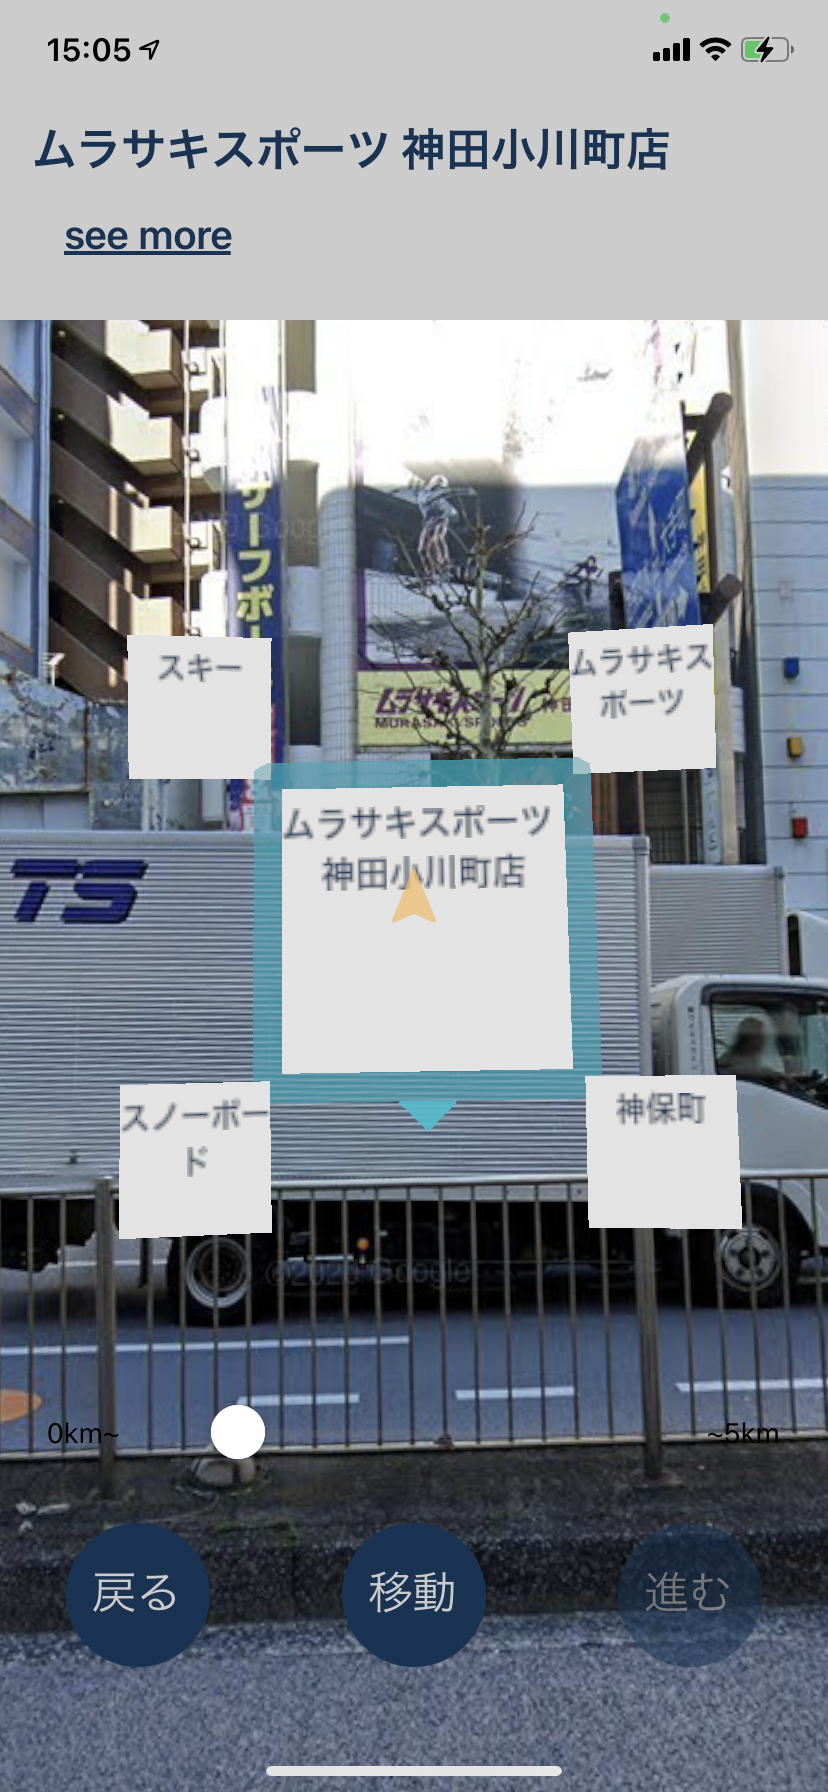
\includegraphics[width=70mm]{images/ar_navigation_jibotyo_ski.png}
    \caption{スキー用品店を選択した時} \label{fig:ar_navigation_jibotyo_ski}
  \end{minipage}
  \begin{minipage}{0.5\hsize}
    \centering
    
\includegraphics[width=70mm]{images/wip2.jpg}
    \caption{飲食店を選択した時} \label{fig:ar_navigation_jibotyo_lunch}
  \end{minipage}
\end{figure}


\section{学習教材としての利用}
wikiはwikipediaに代表されるように膨大な史実や地理情報を整理し、記録するのに適したメディアであると言える。
本システムではwikiの各ページに位置情報を貼り付けるだけでARでの表示を実現できるためこのような地理情報を含む歴史や地理の教材として利用することが可能である。

例として京都などの史跡が多い地域でフィールドワークを行う際に利用することなどが考えられる。
学習者は各地にあるタグに触れるだけで周辺にある史跡の情報見ることができるだけでなく、選択した史跡の関連情報から他の史跡の情報や位置をARで見ることができる。
こうすることで自身の興味や学習対象に関連する史跡を効率よく回り、自身の知らない史跡を知る切っ掛けにもなると考える。

さらに本システムでは第3章で述べた通り現在地からのAR表示だけでなく選択されたAR情報の場所に視点を移動する事が可能である。
この機能によって実際の場所にいなくとも関連情報を元に視点を切り替えながら史跡を見ることが可能である。

\section{リンクを利用した柔軟な記法}
\label{link_enum_notation}
本システムでは位置情報を記載したScrapboxページを作成することでAR情報を登録することができるが、それに加えて、登録されたAR情報のリンクを利用したページを作ることも可能である。
例えば渋谷からSFCのキャンパスまでの経路を記述したい場合は図\ref{fig:route_scrapbox}のように登録した場所などの情報のリンクを利用して記載することができる。
このようにリンクを並べて配置するだけで図(準備中)のように通るべきポイントがARで表示される。
この書き方はユーザによって簡単に行えるだけでなく、並べるリンクが合っていれば表記の揺れにも強いという利点を持っている。

\begin{figure}[h]
  \centering
  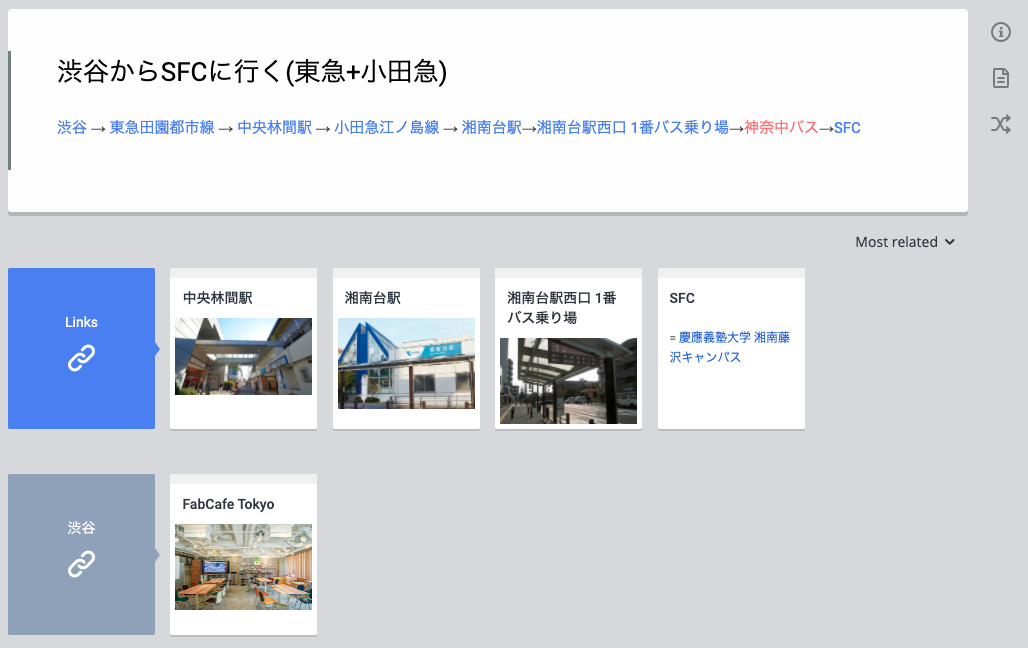
\includegraphics[width=150mm]{images/route_scrapbox.png}
  \caption{リンクを利用したルートの表記例} \label{fig:route_scrapbox}
\end{figure}


\section{まとめ}
本章では、本システムによって実現可能な、NFCタグによるインタラクションとリンクによる関連情報の表示等の機能を活かした利用例について述べた。
タッチというわかりやすいインタラクション、Wikiの持つ拡張性などから、本章で述べた利用例に限らず様々な応用が可能であると考えられる。